\chapter{Selecting Plasma Profiles}

\label{chapter:profiles}

\begin{figure*}[h]
    \centering
    \hfill 
    \begin{subfigure}[t]{0.45\textwidth}
        \centering
		\begin{adjustbox}{width=\textwidth}
			\Large
			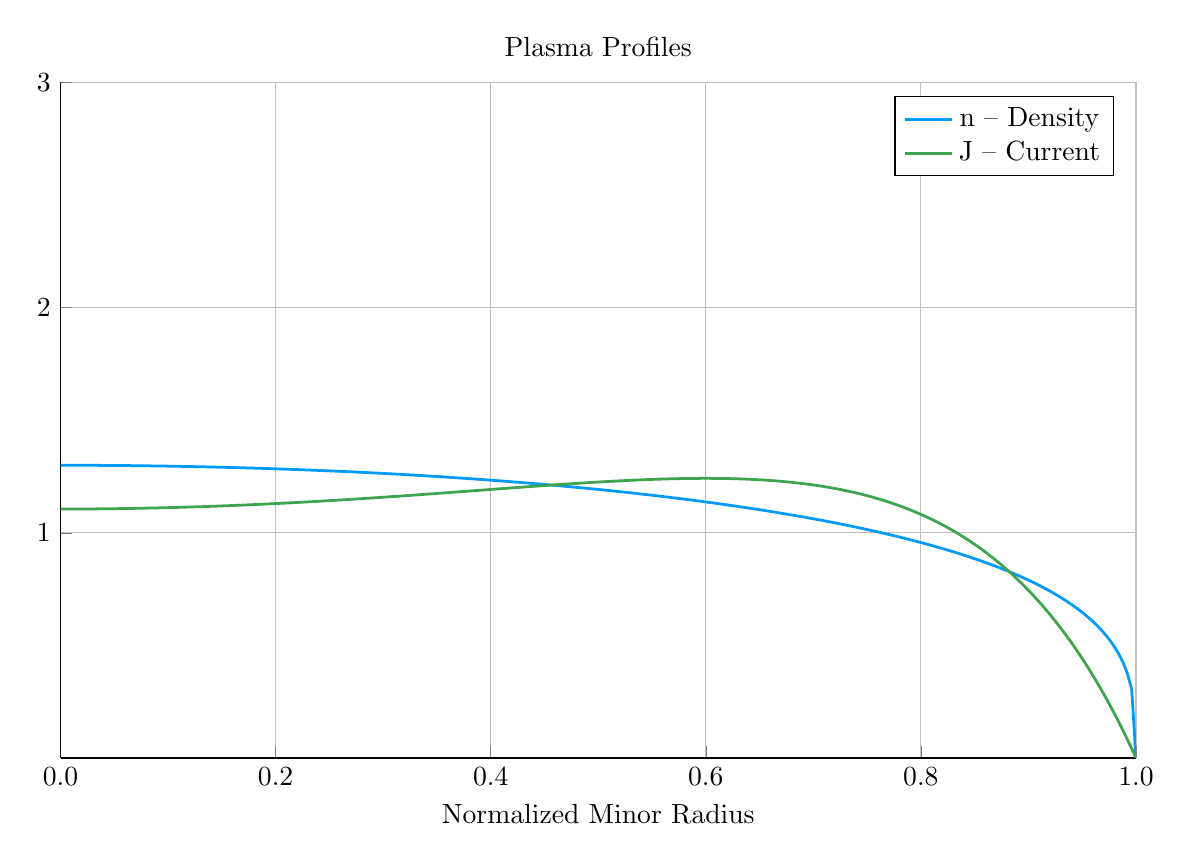
\begin{tikzpicture}[]
\begin{axis}[height = {101.6mm}, ylabel = {}, title = {Plasma Profiles}, xmin = {0.0}, xmax = {1.0}, ymax = {3}, xlabel = {Normalized Minor Radius}, {unbounded coords=jump, scaled x ticks = false, xticklabel style={rotate = 0}, xmajorgrids = true, xtick = {0.0,0.2,0.4,0.6000000000000001,0.8,1.0}, xticklabels = {0.0,0.2,0.4,0.6,0.8,1.0}, xtick align = inside, axis lines* = left, scaled y ticks = false, yticklabel style={rotate = 0}, ymajorgrids = true, ytick = {1.0,2.0,3.0}, yticklabels = {1,2,3}, ytick align = inside, axis lines* = left,     xshift = 0.0mm,
    yshift = 0.0mm,
    axis background/.style={fill={rgb,1:red,1.00000000;green,1.00000000;blue,1.00000000}}
}, ymin = {0}, width = {152.4mm}]\addplot+ [color = {rgb,1:red,0.00000000;green,0.60560316;blue,0.97868012},
draw opacity=1.0,
line width=1,
solid,mark = none,
mark size = 2.0,
mark options = {
    color = {rgb,1:red,0.00000000;green,0.00000000;blue,0.00000000}, draw opacity = 1.0,
    fill = {rgb,1:red,0.00000000;green,0.60560316;blue,0.97868012}, fill opacity = 1.0,
    line width = 1,
    rotate = 0,
    solid
}]coordinates {
(0.0, 1.3)
(0.004, 1.2999937599650557)
(0.008, 1.2999750394408758)
(0.012, 1.299943837169305)
(0.016, 1.2999001510530381)
(0.02, 1.2998439781550484)
(0.024, 1.2997753146977886)
(0.028, 1.2996941560621622)
(0.032, 1.2996004967862647)
(0.036, 1.2994943305638946)
(0.04, 1.2993756502428317)
(0.044, 1.2992444478228855)
(0.048, 1.2991007144537061)
(0.052, 1.2989444404323625)
(0.056, 1.2987756152006849)
(0.06, 1.2985942273423656)
(0.064, 1.2984002645798236)
(0.068, 1.2981937137708253)
(0.072, 1.2979745609048603)
(0.076, 1.2977427910992743)
(0.08, 1.2974983885951488)
(0.084, 1.2972413367529347)
(0.088, 1.2969716180478277)
(0.092, 1.2966892140648891)
(0.096, 1.2963941054939072)
(0.1, 1.2960862721239934)
(0.104, 1.2957656928379149)
(0.108, 1.2954323456061552)
(0.112, 1.295086207480701)
(0.116, 1.2947272545885533)
(0.12, 1.2943554621249538)
(0.124, 1.2939708043463278)
(0.128, 1.2935732545629344)
(0.132, 1.2931627851312222)
(0.136, 1.2927393674458851)
(0.14, 1.2923029719316104)
(0.144, 1.2918535680345185)
(0.148, 1.2913911242132843)
(0.152, 1.290915607929936)
(0.156, 1.2904269856403272)
(0.16, 1.2899252227842701)
(0.164, 1.289410283775332)
(0.168, 1.2888821319902795)
(0.172, 1.2883407297581677)
(0.176, 1.2877860383490682)
(0.18, 1.2872180179624235)
(0.184, 1.286636627715024)
(0.188, 1.286041825628597)
(0.192, 1.2854335686170009)
(0.196, 1.2848118124730112)
(0.2, 1.2841765118546966)
(0.204, 1.2835276202713661)
(0.208, 1.2828650900690854)
(0.212, 1.2821888724157464)
(0.216, 1.2814989172856817)
(0.22, 1.2807951734438123)
(0.224, 1.280077588429316)
(0.228, 1.2793461085388045)
(0.232, 1.2786006788089976)
(0.236, 1.2778412429988808)
(0.24, 1.2770677435713307)
(0.244, 1.2762801216741988)
(0.248, 1.275478317120833)
(0.252, 1.274662268370027)
(0.256, 1.2738319125053779)
(0.26, 1.2729871852140369)
(0.264, 1.2721280207648382)
(0.268, 1.2712543519857844)
(0.272, 1.2703661102408716)
(0.276, 1.2694632254062383)
(0.28, 1.268545625845612)
(0.284, 1.2676132383850391)
(0.288, 1.266665988286872)
(0.292, 1.2657037992229945)
(0.296, 1.2647265932472596)
(0.3, 1.2637342907671185)
(0.304, 1.262726810514414)
(0.308, 1.261704069515311)
(0.312, 1.2606659830593416)
(0.316, 1.2596124646675324)
(0.32, 1.2585434260595858)
(0.324, 1.257458777120088)
(0.328, 1.256358425863706)
(0.332, 1.2552422783993482)
(0.336, 1.2541102388932475)
(0.34, 1.2529622095309358)
(0.344, 1.2517980904780717)
(0.348, 1.2506177798400802)
(0.352, 1.24942117362057)
(0.356, 1.248208165678479)
(0.36, 1.2469786476839106)
(0.364, 1.2457325090726121)
(0.368, 1.2444696369990487)
(0.372, 1.2431899162880222)
(0.376, 1.2418932293847857)
(0.38, 1.2405794563035972)
(0.384, 1.239248474574658)
(0.388, 1.237900159189375)
(0.392, 1.2365343825438908)
(0.396, 1.2351510143808089)
(0.4, 1.2337499217290562)
(0.404, 1.2323309688418065)
(0.408, 1.2308940171323957)
(0.412, 1.229438925108151)
(0.416, 1.2279655483020526)
(0.42, 1.2264737392021483)
(0.424, 1.2249633471786308)
(0.428, 1.2234342184084848)
(0.432, 1.221886195797614)
(0.436, 1.2203191189003393)
(0.44, 1.2187328238361723)
(0.444, 1.2171271432037454)
(0.448, 1.2155019059917886)
(0.452, 1.2138569374870312)
(0.456, 1.212192059178898)
(0.46, 1.210507088660872)
(0.464, 1.208801839528379)
(0.468, 1.2070761212730492)
(0.472, 1.205329739173201)
(0.476, 1.2035624941803869)
(0.48, 1.2017741828018271)
(0.484, 1.1999645969785544)
(0.488, 1.1981335239590802)
(0.492, 1.1962807461683858)
(0.496, 1.1944060410720247)
(0.5, 1.1925091810351223)
(0.504, 1.190589933176035)
(0.508, 1.1886480592144295)
(0.512, 1.1866833153135188)
(0.516, 1.1846954519161883)
(0.52, 1.1826842135747218)
(0.524, 1.1806493387738237)
(0.528, 1.1785905597466213)
(0.532, 1.1765076022833005)
(0.536, 1.1744001855320279)
(0.54, 1.1722680217917714)
(0.544, 1.1701108162966227)
(0.548, 1.1679282669911981)
(0.552, 1.1657200642966656)
(0.556, 1.1634858908669246)
(0.56, 1.1612254213344295)
(0.564, 1.1589383220451273)
(0.568, 1.1566242507819302)
(0.572, 1.154282856476133)
(0.576, 1.1519137789061165)
(0.58, 1.1495166483826693)
(0.584, 1.1470910854201908)
(0.588, 1.1446367003930078)
(0.592, 1.142153093175977)
(0.596, 1.1396398527684999)
(0.6, 1.1370965569010092)
(0.604, 1.1345227716229302)
(0.608, 1.1319180508710498)
(0.612, 1.1292819360171518)
(0.616, 1.1266139553937018)
(0.62, 1.123913623796276)
(0.624, 1.1211804419613376)
(0.628, 1.1184138960178658)
(0.632, 1.1156134569112315)
(0.636, 1.1127785797976015)
(0.64, 1.1099087034070205)
(0.644, 1.1070032493731854)
(0.648, 1.1040616215277776)
(0.652, 1.1010832051570543)
(0.656, 1.0980673662182174)
(0.66, 1.0950134505129014)
(0.664, 1.0919207828148862)
(0.668, 1.0887886659489356)
(0.672, 1.0856163798173906)
(0.676, 1.082403180370883)
(0.68, 1.0791482985192302)
(0.684, 1.075850938978235)
(0.688, 1.0725102790477619)
(0.692, 1.0691254673160542)
(0.696, 1.0656956222848162)
(0.7, 1.0622198309091082)
(0.704, 1.0586971470455604)
(0.708, 1.055126589801824)
(0.712, 1.0515071417795323)
(0.716, 1.04783774720231)
(0.72, 1.0441173099195802)
(0.724, 1.0403446912760228)
(0.728, 1.03651870783555)
(0.732, 1.0326381289475657)
(0.736, 1.0287016741420443)
(0.74, 1.0247080103385948)
(0.744, 1.0206557488531367)
(0.748, 1.0165434421840995)
(0.752, 1.0123695805581145)
(0.756, 1.0081325882130072)
(0.76, 1.003830819393436)
(0.764, 0.9994625540317649)
(0.768, 0.9950259930836299)
(0.772, 0.990519253484107)
(0.776, 0.9859403626863661)
(0.78, 0.9812872527401133)
(0.784, 0.9765577538618856)
(0.788, 0.9717495874432898)
(0.792, 0.9668603584364187)
(0.796, 0.9618875470478029)
(0.8, 0.9568284996631833)
(0.804, 0.9516804189149115)
(0.808, 0.946440352791649)
(0.812, 0.9411051826759365)
(0.816, 0.9356716101787849)
(0.82, 0.9301361426212457)
(0.824, 0.9244950769904182)
(0.828, 0.9187444821708816)
(0.832, 0.9128801792212949)
(0.836, 0.9068977194288869)
(0.84, 0.900792359830521)
(0.844, 0.8945590358364464)
(0.848, 0.8881923305297794)
(0.852, 0.8816864401388146)
(0.856, 0.8750351350873486)
(0.86, 0.8682317159164477)
(0.864, 0.86126896323448)
(0.868, 0.8541390806843802)
(0.872, 0.8468336297096526)
(0.876, 0.8393434546426821)
(0.88, 0.8316585963161566)
(0.884, 0.8237681919917861)
(0.888, 0.81566035888456)
(0.892, 0.8073220579010558)
(0.896, 0.7987389333598728)
(0.9, 0.7898951233563103)
(0.904, 0.7807730339816926)
(0.908, 0.7713530686829113)
(0.912, 0.7616133014678136)
(0.916, 0.7515290791633757)
(0.92, 0.7410725331284098)
(0.924, 0.7302119741312908)
(0.928, 0.7189111346441375)
(0.932, 0.7071282092103691)
(0.936, 0.6948146236457978)
(0.94, 0.6819134341198397)
(0.944, 0.6683572117823803)
(0.948, 0.654065197526229)
(0.952, 0.6389393969490827)
(0.956, 0.6228590949732707)
(0.96, 0.6056729403361176)
(0.964, 0.5871871562979527)
(0.968, 0.5671473067124922)
(0.972, 0.5452087722509604)
(0.976, 0.520886146278826)
(0.98, 0.4934599473688843)
(0.984, 0.46178715390262587)
(0.988, 0.4238602013900372)
(0.992, 0.3755408186191309)
(0.996, 0.3052175562338072)
(1.0, 0.0)
};
\addlegendentry{n -- Density}
\addplot+ [color = {rgb,1:red,0.24222430;green,0.64327509;blue,0.30444865},
draw opacity=1.0,
line width=1,
solid,mark = none,
mark size = 2.0,
mark options = {
    color = {rgb,1:red,0.00000000;green,0.00000000;blue,0.00000000}, draw opacity = 1.0,
    fill = {rgb,1:red,0.24222430;green,0.64327509;blue,0.30444865}, fill opacity = 1.0,
    line width = 1,
    rotate = 0,
    solid
}]coordinates {
(0.0, 1.1055925931810484)
(0.004, 1.1056025434176453)
(0.008, 1.105632392966404)
(0.012, 1.1056821383432776)
(0.016, 1.1057517737383413)
(0.02, 1.1058412910110205)
(0.024, 1.1059506796834087)
(0.028, 1.106079926931665)
(0.032, 1.106229017575493)
(0.036, 1.1063979340656915)
(0.04, 1.106586656469768)
(0.044, 1.1067951624556105)
(0.048, 1.107023427273207)
(0.052, 1.1072714237343937)
(0.056, 1.1075391221906397)
(0.06, 1.107826490508826)
(0.064, 1.1081334940450354)
(0.068, 1.1084600956163122)
(0.072, 1.1088062554703932)
(0.076, 1.1091719312533783)
(0.08, 1.1095570779753314)
(0.084, 1.1099616479737875)
(0.088, 1.110385590875139)
(0.092, 1.1108288535538926)
(0.096, 1.1112913800897515)
(0.1, 1.1117731117225211)
(0.104, 1.1122739868047913)
(0.108, 1.112793940752376)
(0.112, 1.1133329059924844)
(0.116, 1.1138908119095834)
(0.12, 1.1144675847889256)
(0.124, 1.115063147757707)
(0.128, 1.1156774207238216)
(0.132, 1.1163103203121705)
(0.136, 1.1169617597984949)
(0.14, 1.1176316490406888)
(0.144, 1.11831989440755)
(0.148, 1.119026398704931)
(0.152, 1.11975106109924)
(0.156, 1.120493777038251)
(0.16, 1.1212544381691738)
(0.164, 1.1220329322539315)
(0.168, 1.1228291430816038)
(0.172, 1.1236429503779706)
(0.176, 1.1244742297121144)
(0.18, 1.1253228524000167)
(0.184, 1.1261886854050946)
(0.188, 1.127071591235615)
(0.192, 1.1279714278389303)
(0.196, 1.128888048492462)
(0.2, 1.1298213016913794)
(0.204, 1.1307710310328927)
(0.208, 1.131737075097102)
(0.212, 1.1327192673243216)
(0.216, 1.1337174358888118)
(0.22, 1.1347314035688367)
(0.224, 1.135760987612975)
(0.228, 1.136805999602598)
(0.232, 1.1378662453104351)
(0.236, 1.1389415245551366)
(0.24, 1.140031631051753)
(0.244, 1.1411363522580324)
(0.248, 1.1422554692164475)
(0.252, 1.143388756391854)
(0.256, 1.1445359815046836)
(0.26, 1.145696905359567)
(0.264, 1.146871281669287)
(0.268, 1.1480588568739498)
(0.272, 1.1492593699552682)
(0.276, 1.1504725522458386)
(0.28, 1.1516981272333027)
(0.284, 1.1529358103592642)
(0.288, 1.1541853088128475)
(0.292, 1.1554463213187653)
(0.296, 1.1567185379197655)
(0.3, 1.15800163975333)
(0.304, 1.1592952988224805)
(0.308, 1.160599177760553)
(0.312, 1.1619129295898027)
(0.316, 1.1632361974736778)
(0.32, 1.1645686144626213)
(0.324, 1.1659098032332398)
(0.328, 1.1672593758206753)
(0.332, 1.1686169333440195)
(0.336, 1.1699820657245965)
(0.34, 1.171354351396943)
(0.344, 1.1727333570123062)
(0.348, 1.1741186371344703)
(0.352, 1.1755097339277303)
(0.356, 1.176906176836817)
(0.36, 1.1783074822585666)
(0.364, 1.1797131532051435)
(0.368, 1.181122678958593)
(0.372, 1.1825355347165192)
(0.376, 1.1839511812286583)
(0.38, 1.1853690644241248)
(0.384, 1.1867886150290958)
(0.388, 1.1882092481746926)
(0.392, 1.1896303629948166)
(0.396, 1.1910513422136817)
(0.4, 1.1924715517227884)
(0.404, 1.1938903401470713)
(0.408, 1.1953070383999467)
(0.412, 1.1967209592269779)
(0.416, 1.198131396737873)
(0.42, 1.199537625926516)
(0.424, 1.2009389021787291)
(0.428, 1.2023344607674524)
(0.432, 1.2037235163350242)
(0.436, 1.205105262362225)
(0.44, 1.2064788706237588)
(0.444, 1.2078434906298132)
(0.448, 1.2091982490533475)
(0.452, 1.2105422491427469)
(0.456, 1.2118745701194584)
(0.46, 1.2131942665602276)
(0.464, 1.2145003677635429)
(0.468, 1.2157918770998737)
(0.472, 1.2170677713452926)
(0.476, 1.218326999998044)
(0.48, 1.219568484577629)
(0.484, 1.220791117905943)
(0.488, 1.2219937633700142)
(0.492, 1.2231752541658545)
(0.496, 1.2243343925229389)
(0.5, 1.2254699489088112)
(0.504, 1.2265806612132972)
(0.508, 1.227665233911794)
(0.512, 1.2287223372070952)
(0.516, 1.229750606149186)
(0.52, 1.2307486397324405)
(0.524, 1.2317149999696246)
(0.528, 1.2326482109421029)
(0.532, 1.2335467578256245)
(0.536, 1.234409085891052)
(0.54, 1.235233599479366)
(0.544, 1.2360186609502908)
(0.548, 1.2367625896038223)
(0.552, 1.2374636605739702)
(0.556, 1.2381201036939686)
(0.56, 1.2387301023322053)
(0.564, 1.2392917921981084)
(0.568, 1.2398032601171822)
(0.572, 1.2402625427743916)
(0.576, 1.2406676254250506)
(0.58, 1.241016440572357)
(0.584, 1.2413068666106932)
(0.588, 1.2415367264337844)
(0.592, 1.2417037860067774)
(0.596, 1.2418057529012922)
(0.6, 1.2418402747924557)
(0.604, 1.2418049379169072)
(0.608, 1.2416972654907381)
(0.612, 1.2415147160863034)
(0.616, 1.2412546819667964)
(0.62, 1.2409144873774753)
(0.624, 1.24049138679237)
(0.628, 1.2399825631152874)
(0.632, 1.239385125833895)
(0.636, 1.2386961091256128)
(0.64, 1.2379124699140391)
(0.644, 1.2370310858745734)
(0.648, 1.2360487533878732)
(0.652, 1.2349621854397481)
(0.656, 1.233768009466043)
(0.66, 1.2324627651410391)
(0.664, 1.2310429021078442)
(0.668, 1.2295047776492094)
(0.672, 1.2278446542971666)
(0.676, 1.2260586973798364)
(0.68, 1.224142972503699)
(0.684, 1.2220934429695933)
(0.688, 1.219905967120643)
(0.692, 1.2175762956202625)
(0.696, 1.2151000686583564)
(0.7, 1.2124728130837497)
(0.704, 1.2096899394608527)
(0.708, 1.206746739048499)
(0.712, 1.2036383806988336)
(0.716, 1.200359907674078)
(0.72, 1.1969062343789294)
(0.724, 1.1932721430062943)
(0.728, 1.1894522800939817)
(0.732, 1.1854411529899347)
(0.736, 1.181233126223481)
(0.74, 1.1768224177800433)
(0.744, 1.172203095276651)
(0.748, 1.1673690720355396)
(0.752, 1.162314103053033)
(0.756, 1.1570317808608346)
(0.76, 1.1515155312767646)
(0.764, 1.1457586090418983)
(0.768, 1.1397540933409778)
(0.772, 1.133494883202872)
(0.776, 1.1269736927777798)
(0.78, 1.1201830464877607)
(0.784, 1.1131152740470984)
(0.788, 1.1057625053488873)
(0.792, 1.0981166652141365)
(0.796, 1.0901694679995795)
(0.8, 1.0819124120602648)
(0.804, 1.0733367740628939)
(0.808, 1.064433603145756)
(0.812, 1.0551937149209845)
(0.816, 1.0456076853147525)
(0.82, 1.0356658442408755)
(0.824, 1.0253582691031793)
(0.828, 1.0146747781218477)
(0.832, 1.0036049234788245)
(0.836, 0.99213798427721)
(0.84, 0.980262959309437)
(0.844, 0.9679685596288679)
(0.848, 0.9552432009192925)
(0.852, 0.9420749956566505)
(0.856, 0.9284517450571373)
(0.86, 0.9143609308056804)
(0.864, 0.8997897065585966)
(0.868, 0.8847248892140719)
(0.872, 0.8691529499438978)
(0.876, 0.8530600049797328)
(0.88, 0.8364318061469402)
(0.884, 0.819253731138866)
(0.888, 0.8015107735241939)
(0.892, 0.783187532479819)
(0.896, 0.7642682022414483)
(0.9, 0.7447365612639053)
(0.904, 0.72457596108289)
(0.908, 0.7037693148696959)
(0.912, 0.6822990856701381)
(0.916, 0.6601472743186879)
(0.92, 0.6372954070185461)
(0.924, 0.6137245225781115)
(0.928, 0.5894151592940192)
(0.932, 0.564347341470635)
(0.936, 0.5385005655655922)
(0.94, 0.5118537859506463)
(0.944, 0.48438540027680593)
(0.948, 0.45607323443237957)
(0.952, 0.4268945270822218)
(0.956, 0.39682591377612964)
(0.96, 0.3658434106139833)
(0.964, 0.3339223974548356)
(0.968, 0.30103760065679763)
(0.972, 0.2671630753341644)
(0.976, 0.23227218711781)
(0.98, 0.19633759340448617)
(0.984, 0.15933122408020503)
(0.988, 0.12122426170246466)
(0.992, 0.08198712112559489)
(0.996, 0.04158942855305283)
(1.0, 0.0)
};
\addlegendentry{J -- Current}
\end{axis}

\end{tikzpicture}

		\end{adjustbox}
        \caption{Density and Current Profiles}
    \end{subfigure}
    \hfill
    \begin{subfigure}[t]{0.45\textwidth}
        \centering
		\begin{adjustbox}{width=\textwidth}
			\Large
			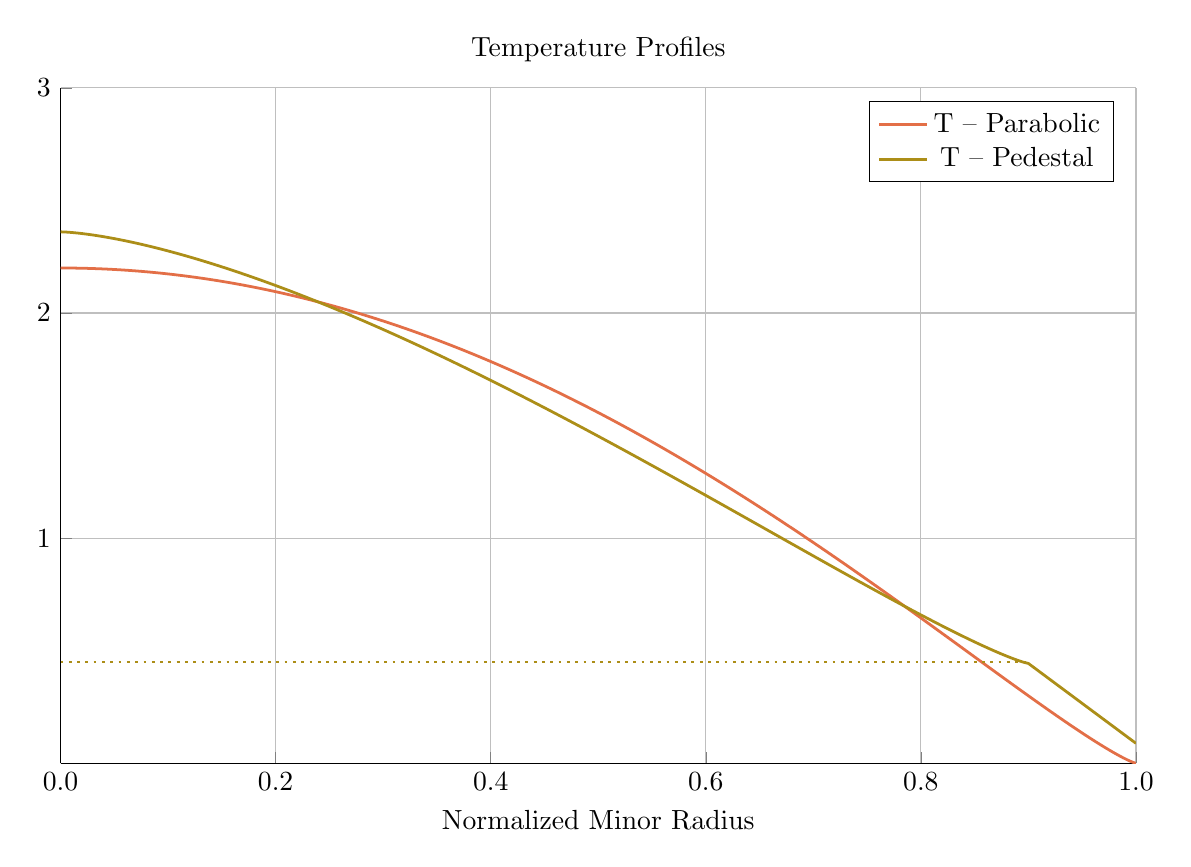
\begin{tikzpicture}[]
\begin{axis}[height = {101.6mm}, ylabel = {}, title = {Temperature Profiles}, xmin = {0.0}, xmax = {1.0}, ymax = {3}, xlabel = {Normalized Minor Radius}, {unbounded coords=jump, scaled x ticks = false, xticklabel style={rotate = 0}, xmajorgrids = true, xtick = {0.0,0.2,0.4,0.6000000000000001,0.8,1.0}, xticklabels = {0.0,0.2,0.4,0.6,0.8,1.0}, xtick align = inside, axis lines* = left, scaled y ticks = false, yticklabel style={rotate = 0}, ymajorgrids = true, ytick = {1.0,2.0,3.0}, yticklabels = {1,2,3}, ytick align = inside, axis lines* = left,     xshift = 0.0mm,
    yshift = 0.0mm,
    axis background/.style={fill={rgb,1:red,1.00000000;green,1.00000000;blue,1.00000000}}
}, ymin = {0}, width = {152.4mm}]\addplot+ [color = {rgb,1:red,0.88887350;green,0.43564919;blue,0.27812294},
draw opacity=1.0,
line width=1,
solid,mark = none,
mark size = 2.0,
mark options = {
    color = {rgb,1:red,0.00000000;green,0.00000000;blue,0.00000000}, draw opacity = 1.0,
    fill = {rgb,1:red,0.88887350;green,0.43564919;blue,0.27812294}, fill opacity = 1.0,
    line width = 1,
    rotate = 0,
    solid
}]coordinates {
(0.0, 2.2)
(0.004, 2.1999577600675844)
(0.008, 2.199831041081363)
(0.012, 2.199619845474514)
(0.016, 2.1993241773026853)
(0.02, 2.198944042244507)
(0.024, 2.1984794476023213)
(0.028, 2.1979304023031214)
(0.032, 2.1972969168996905)
(0.036, 2.196579003571959)
(0.04, 2.195776676128566)
(0.044, 2.194889950008634)
(0.048, 2.1939188422837517)
(0.052, 2.192863371660171)
(0.056, 2.1917235584812182)
(0.06, 2.1904994247299143)
(0.064, 2.189190994031813)
(0.068, 2.187798291658056)
(0.072, 2.1863213445286407)
(0.076, 2.1847601812159145)
(0.08, 2.1831148319482794)
(0.084, 2.1813853286141245)
(0.088, 2.179571704765981)
(0.092, 2.1776739956248985)
(0.096, 2.1756922380850554)
(0.1, 2.1736264707185855)
(0.104, 2.1714767337806498)
(0.108, 2.1692430692147298)
(0.112, 2.1669255206581606)
(0.116, 2.164524133447901)
(0.12, 2.1620389546265417)
(0.124, 2.1594700329485588)
(0.128, 2.1568174188868077)
(0.132, 2.154081164639269)
(0.136, 2.1512613241360428)
(0.14, 2.148357953046596)
(0.144, 2.1453711087872693)
(0.148, 2.1423008505290397)
(0.152, 2.139147239205551)
(0.156, 2.1359103375214086)
(0.16, 2.1325902099607443)
(0.164, 2.129186922796058)
(0.168, 2.1257005440973358)
(0.172, 2.1221311437414503)
(0.176, 2.1184787934218474)
(0.18, 2.1147435666585284)
(0.184, 2.1109255388083183)
(0.188, 2.1070247870754453)
(0.192, 2.1030413905224172)
(0.196, 2.098975430081212)
(0.2, 2.09482698856478)
(0.204, 2.090596150678874)
(0.208, 2.086283003034196)
(0.212, 2.0818876341588837)
(0.216, 2.0774101345113314)
(0.22, 2.072850596493357)
(0.224, 2.068209114463716)
(0.228, 2.063485784751976)
(0.232, 2.058680705672756)
(0.236, 2.053793977540332)
(0.24, 2.0488257026836245)
(0.244, 2.043775985461571)
(0.248, 2.038644932278893)
(0.252, 2.033432651602259)
(0.256, 2.0281392539768675)
(0.26, 2.022764852043437)
(0.264, 2.0173095605556335)
(0.268, 2.0117734963979244)
(0.272, 2.006156778603888)
(0.276, 2.0004595283749724)
(0.28, 1.9946818690997206)
(0.284, 1.9888239263734737)
(0.288, 1.9828858280185606)
(0.292, 1.976867704104986)
(0.296, 1.9707696869716258)
(0.3, 1.9645919112479475)
(0.304, 1.9583345138762616)
(0.308, 1.9519976341345224)
(0.312, 1.9455814136596863)
(0.316, 1.939085996471644)
(0.32, 1.932511528997742)
(0.324, 1.9258581600979061)
(0.328, 1.9191260410903783)
(0.332, 1.912315325778094)
(0.336, 1.9054261704757012)
(0.34, 1.8984587340372499)
(0.344, 1.8914131778845642)
(0.348, 1.8842896660363146)
(0.352, 1.8770883651378103)
(0.356, 1.8698094444915332)
(0.36, 1.8624530760884261)
(0.364, 1.8550194346399664)
(0.368, 1.8475086976110369)
(0.372, 1.839921045253621)
(0.376, 1.8322566606413475)
(0.38, 1.8245157297049002)
(0.384, 1.8166984412683274)
(0.388, 1.8088049870862715)
(0.392, 1.8008355618821434)
(0.396, 1.792790363387276)
(0.4, 1.7846695923810785)
(0.404, 1.776473452732227)
(0.408, 1.7682021514409176)
(0.412, 1.7598558986822177)
(0.416, 1.7514349078505493)
(0.42, 1.742939395605332)
(0.424, 1.7343695819178346)
(0.428, 1.725725690119258)
(0.432, 1.7170079469501018)
(0.436, 1.7082165826108464)
(0.44, 1.6993518308139948)
(0.444, 1.6904139288375197)
(0.448, 1.6814031175797635)
(0.452, 1.6723196416158315)
(0.456, 1.6631637492555364)
(0.46, 1.653935692602939)
(0.464, 1.6446357276175452)
(0.468, 1.6352641141772097)
(0.472, 1.6258211161428078)
(0.476, 1.6163070014247378)
(0.48, 1.606722042051314)
(0.484, 1.5970665142391203)
(0.488, 1.5873406984653924)
(0.492, 1.5775448795424998)
(0.496, 1.5676793466946068)
(0.5, 1.5577443936365882)
(0.504, 1.5477403186552856)
(0.508, 1.5376674246931867)
(0.512, 1.5275260194346267)
(0.516, 1.517316415394591)
(0.52, 1.5070389300102414)
(0.524, 1.4966938857352434)
(0.528, 1.4862816101370295)
(0.532, 1.4758024359970894)
(0.536, 1.465256701414425)
(0.54, 1.4546447499122863)
(0.544, 1.4439669305483216)
(0.548, 1.4332235980282817)
(0.552, 1.4224151128234246)
(0.556, 1.4115418412917677)
(0.56, 1.4006041558033582)
(0.564, 1.3896024348697198)
(0.568, 1.3785370632776597)
(0.572, 1.3674084322276236)
(0.576, 1.3562169394767907)
(0.58, 1.3449629894871216)
(0.584, 1.333646993578575)
(0.588, 1.3222693700877242)
(0.592, 1.3108305445320172)
(0.596, 1.2993309497799401)
(0.6, 1.2877710262273512)
(0.604, 1.2761512219802742)
(0.608, 1.2644719930444575)
(0.612, 1.2527338035220144)
(0.616, 1.2409371258154922)
(0.62, 1.2290824408397232)
(0.624, 1.2171702382418437)
(0.628, 1.2052010166298843)
(0.632, 1.1931752838103635)
(0.636, 1.1810935570353371)
(0.64, 1.1689563632593918)
(0.644, 1.156764239407098)
(0.648, 1.1445177326514693)
(0.652, 1.1322174007040144)
(0.656, 1.1198638121170017)
(0.66, 1.1074575465986056)
(0.664, 1.0949991953416336)
(0.668, 1.082489361366603)
(0.672, 1.0699286598799627)
(0.676, 1.0573177186483342)
(0.68, 1.044657178389695)
(0.684, 1.0319476931824922)
(0.688, 1.019189930893753)
(0.692, 1.0063845736273342)
(0.696, 0.9935323181935332)
(0.7, 0.980633876601379)
(0.704, 0.9676899765750238)
(0.708, 0.9547013620957563)
(0.712, 0.9416687939712927)
(0.716, 0.9285930504341149)
(0.72, 0.9154749277707805)
(0.724, 0.9023152409842818)
(0.728, 0.8891148244917015)
(0.732, 0.8758745328596077)
(0.736, 0.8625952415798288)
(0.74, 0.849277847888491)
(0.744, 0.8359232716314423)
(0.748, 0.822532456179475)
(0.752, 0.8091063693970627)
(0.756, 0.7956460046686752)
(0.76, 0.7821523819871128)
(0.764, 0.7686265491087244)
(0.768, 0.7550695827808527)
(0.772, 0.7414825900473649)
(0.776, 0.7278667096387308)
(0.78, 0.7142231134537544)
(0.784, 0.7005530081408239)
(0.788, 0.6868576367873601)
(0.792, 0.6731382807270975)
(0.796, 0.6593962614758839)
(0.8, 0.6456329428078906)
(0.804, 0.6318497329854856)
(0.808, 0.6180480871575735)
(0.812, 0.6042295099429783)
(0.816, 0.5903955582174578)
(0.82, 0.5765478441252689)
(0.824, 0.5626880383388612)
(0.828, 0.5488178735933505)
(0.832, 0.5349391485259877)
(0.836, 0.5210537318549578)
(0.84, 0.5071635669366619)
(0.844, 0.49327067674623953)
(0.848, 0.47937716933269775)
(0.852, 0.46548524380775297)
(0.856, 0.45159719693668826)
(0.86, 0.4377154304104124)
(0.864, 0.42384245889091393)
(0.868, 0.40998091893787963)
(0.872, 0.3961335789430169)
(0.876, 0.38230335022134865)
(0.88, 0.36849329943642983)
(0.884, 0.35470666257034567)
(0.888, 0.340946860691165)
(0.892, 0.3272175178224195)
(0.896, 0.31352248128407095)
(0.9, 0.2998658449561726)
(0.904, 0.28625197602028446)
(0.908, 0.2726855458667975)
(0.912, 0.25917156602852953)
(0.916, 0.24571543022609155)
(0.92, 0.23232296390814428)
(0.924, 0.21900048306792003)
(0.928, 0.20575486465742054)
(0.932, 0.1925936316637043)
(0.936, 0.17952505695042487)
(0.94, 0.16655829144594192)
(0.944, 0.15370352440467291)
(0.948, 0.14097218665156444)
(0.952, 0.12837721256189286)
(0.956, 0.11593338410667639)
(0.96, 0.10365779254585625)
(0.964, 0.09157047392306764)
(0.968, 0.07969531062880889)
(0.972, 0.06806135815914495)
(0.976, 0.056704888286093984)
(0.98, 0.04567272289384328)
(0.984, 0.035028106493367024)
(0.988, 0.024862215823612335)
(0.992, 0.0153206738078139)
(0.996, 0.0066847830139362754)
(1.0, 0.0)
};
\addlegendentry{T -- Parabolic}
\addplot+ [color = {rgb,1:red,0.67554396;green,0.55566233;blue,0.09423434},
draw opacity=1.0,
line width=1,
solid,mark = none,
mark size = 2.0,
mark options = {
    color = {rgb,1:red,0.00000000;green,0.00000000;blue,0.00000000}, draw opacity = 1.0,
    fill = {rgb,1:red,0.67554396;green,0.55566233;blue,0.09423434}, fill opacity = 1.0,
    line width = 1,
    rotate = 0,
    solid
}]coordinates {
(0.0, 2.3605919704710323)
(0.004, 2.359910398918797)
(0.008, 2.3586642994783618)
(0.012, 2.3570508613498493)
(0.016, 2.3551405297956594)
(0.02, 2.3529740696983454)
(0.024, 2.350579025743975)
(0.028, 2.3479756517769723)
(0.032, 2.3451796682823796)
(0.036, 2.342203747147281)
(0.04, 2.3390583928390996)
(0.044, 2.3357525032801973)
(0.048, 2.332293746279636)
(0.052, 2.328688822918463)
(0.056, 2.3249436581415552)
(0.06, 2.3210635425572748)
(0.064, 2.3170532404255844)
(0.068, 2.3129170735482543)
(0.072, 2.3086589875663335)
(0.076, 2.3042826051438894)
(0.08, 2.299791269197131)
(0.084, 2.295188078444673)
(0.088, 2.2904759169492626)
(0.092, 2.2856574788975115)
(0.096, 2.2807352895619175)
(0.1, 2.2757117231701707)
(0.104, 2.2705890182452353)
(0.108, 2.2653692908590712)
(0.112, 2.260054546151598)
(0.116, 2.2546466883966962)
(0.12, 2.2491475298430212)
(0.124, 2.243558798515241)
(0.128, 2.237882145128044)
(0.132, 2.2321191492388524)
(0.136, 2.2262713247439767)
(0.14, 2.220340124805883)
(0.144, 2.2143269462853388)
(0.148, 2.2082331337408316)
(0.152, 2.202059983048349)
(0.156, 2.1958087446868073)
(0.16, 2.189480626728042)
(0.164, 2.1830767975648464)
(0.168, 2.176598388406032)
(0.172, 2.1700464955636813)
(0.176, 2.163422182554496)
(0.18, 2.1567264820344176)
(0.184, 2.149960397583317)
(0.188, 2.14312490535454)
(0.192, 2.1362209556023704)
(0.196, 2.1292494740989305)
(0.2, 2.1222113634507807)
(0.204, 2.1151075043243255)
(0.208, 2.1079387565881396)
(0.212, 2.1007059603794906)
(0.216, 2.0934099371015487)
(0.22, 2.0860514903571366)
(0.224, 2.0786314068242686)
(0.228, 2.0711504570782133)
(0.232, 2.063609396364366)
(0.236, 2.0560089653257996)
(0.24, 2.0483498906890096)
(0.244, 2.040632885911039)
(0.248, 2.0328586517908898)
(0.252, 2.0250278770478602)
(0.256, 2.0171412388692334)
(0.26, 2.009199403429513)
(0.264, 2.00120302638324)
(0.268, 1.9931527533332325)
(0.272, 1.9850492202759686)
(0.276, 1.97689305402566)
(0.28, 1.9686848726184767)
(0.284, 1.9604252856982425)
(0.288, 1.9521148948848384)
(0.292, 1.9437542941264454)
(0.296, 1.9353440700366855)
(0.3, 1.9268848022176337)
(0.304, 1.9183770635696087)
(0.308, 1.9098214205885893)
(0.312, 1.9012184336520364)
(0.316, 1.8925686572938556)
(0.32, 1.883872640469185)
(0.324, 1.8751309268096423)
(0.328, 1.8663440548696335)
(0.332, 1.8575125583642822)
(0.336, 1.8486369663995004)
(0.34, 1.839717803694704)
(0.344, 1.8307555907986295)
(0.348, 1.8217508442986934)
(0.352, 1.812704077024307)
(0.356, 1.8036157982445404)
(0.36, 1.7944865138605)
(0.364, 1.7853167265927747)
(0.368, 1.776106936164285)
(0.372, 1.7668576394788444)
(0.376, 1.7575693307957496)
(0.38, 1.74824250190067)
(0.384, 1.7388776422731294)
(0.388, 1.7294752392508332)
(0.392, 1.7200357781911024)
(0.396, 1.7105597426296557)
(0.4, 1.7010476144369753)
(0.404, 1.6914998739724885)
(0.408, 1.6819170002367874)
(0.412, 1.6722994710220926)
(0.416, 1.6626477630611856)
(0.42, 1.6529623521750014)
(0.424, 1.6432437134190898)
(0.428, 1.633492321229143)
(0.432, 1.6237086495657764)
(0.436, 1.6138931720587668)
(0.44, 1.6040463621509233)
(0.444, 1.5941686932417938)
(0.448, 1.584260638831387)
(0.452, 1.5743226726641009)
(0.456, 1.5643552688730447)
(0.46, 1.5543589021249482)
(0.464, 1.544334047765842)
(0.468, 1.5342811819677138)
(0.472, 1.5242007818763206)
(0.476, 1.5140933257603746)
(0.48, 1.5039592931622903)
(0.484, 1.4937991650507099)
(0.488, 1.4836134239750187)
(0.492, 1.473402554222062)
(0.496, 1.4631670419753044)
(0.5, 1.4529073754766455)
(0.504, 1.4426240451911474)
(0.508, 1.4323175439749165)
(0.512, 1.4219883672464035)
(0.516, 1.4116370131613858)
(0.52, 1.4012639827919213)
(0.524, 1.3908697803095635)
(0.528, 1.3804549131731465)
(0.532, 1.3700198923214701)
(0.536, 1.359565232371216)
(0.54, 1.349091451820459)
(0.544, 1.3385990732581485)
(0.548, 1.328088623579961)
(0.552, 1.3175606342109392)
(0.556, 1.307015641335371)
(0.56, 1.2964541861343752)
(0.564, 1.2858768150316933)
(0.568, 1.2752840799482301)
(0.572, 1.2646765385659007)
(0.576, 1.2540547546013914)
(0.58, 1.2434192980904786)
(0.584, 1.2327707456835955)
(0.588, 1.222109680953382)
(0.592, 1.211436694715004)
(0.596, 1.200752385360086)
(0.6, 1.1900573592051713)
(0.604, 1.1793522308556705)
(0.608, 1.1686376235863563)
(0.612, 1.1579141697395272)
(0.616, 1.1471825111420575)
(0.62, 1.1364432995426441)
(0.624, 1.1256971970706737)
(0.628, 1.1149448767182386)
(0.632, 1.1041870228469695)
(0.636, 1.093424331721486)
(0.64, 1.0826575120714315)
(0.644, 1.0718872856842108)
(0.648, 1.061114388030769)
(0.652, 1.0503395689269308)
(0.656, 1.039563593233075)
(0.66, 1.0287872415951647)
(0.664, 1.0180113112304485)
(0.668, 1.0072366167614726)
(0.672, 0.9964639911023957)
(0.676, 0.9856942864020085)
(0.68, 0.9749283750483018)
(0.684, 0.9641671507399459)
(0.688, 0.9534115296306018)
(0.692, 0.9426624515526333)
(0.696, 0.9319208813275146)
(0.7, 0.9211878101710503)
(0.704, 0.9104642572024598)
(0.708, 0.8997512710674346)
(0.712, 0.8890499316865009)
(0.716, 0.8783613521413978)
(0.72, 0.8676866807137728)
(0.724, 0.8570271030923351)
(0.728, 0.8463838447667099)
(0.732, 0.8357581736286817)
(0.736, 0.8251514028043623)
(0.74, 0.8145648937441141)
(0.744, 0.8040000596009286)
(0.748, 0.7934583689324995)
(0.752, 0.7829413497675711)
(0.756, 0.7724505940834616)
(0.76, 0.7619877627491815)
(0.764, 0.7515545909975108)
(0.768, 0.741152894500166)
(0.772, 0.7307845761331225)
(0.776, 0.7204516335348546)
(0.78, 0.710156167579369)
(0.784, 0.6999003919093338)
(0.788, 0.6896866437035094)
(0.792, 0.6795173958885602)
(0.796, 0.6693952710502226)
(0.8, 0.6593230573553601)
(0.804, 0.6493037268683398)
(0.808, 0.6393404567373293)
(0.812, 0.6294366538454373)
(0.816, 0.6195959836776518)
(0.82, 0.6098224043609094)
(0.824, 0.6001202071108945)
(0.828, 0.5904940646939226)
(0.832, 0.58094909002811)
(0.836, 0.5714909077694643)
(0.84, 0.562125742755608)
(0.844, 0.5528605306710853)
(0.848, 0.5437030585117963)
(0.852, 0.5346621457948362)
(0.856, 0.5257478827341294)
(0.86, 0.516971950132737)
(0.864, 0.5083480600719166)
(0.868, 0.49989258164201933)
(0.872, 0.4916254625709785)
(0.876, 0.48357164972903754)
(0.88, 0.47576340897240366)
(0.884, 0.4682444150948954)
(0.888, 0.4610777748740693)
(0.892, 0.45436452608473005)
(0.896, 0.44830036952087016)
(0.9, 0.44361517600666117)
(0.904, 0.429419490374448)
(0.908, 0.41522380474223486)
(0.912, 0.4010281191100217)
(0.916, 0.38683243347780855)
(0.92, 0.3726367478455953)
(0.924, 0.3584410622133822)
(0.928, 0.34424537658116894)
(0.932, 0.3300496909489558)
(0.936, 0.3158540053167426)
(0.94, 0.30165831968452983)
(0.944, 0.28746263405231665)
(0.948, 0.27326694842010346)
(0.952, 0.2590712627878903)
(0.956, 0.24487557715567715)
(0.96, 0.23067989152346396)
(0.964, 0.21648420589125078)
(0.968, 0.2022885202590376)
(0.972, 0.18809283462682444)
(0.976, 0.17389714899461126)
(0.98, 0.1597014633623981)
(0.984, 0.14550577773018494)
(0.988, 0.13131009209797176)
(0.992, 0.11711440646575859)
(0.996, 0.1029187208335454)
(1.0, 0.08872303520133223)
};
\addlegendentry{T -- Pedestal}
\addplot+ [color = {rgb,1:red,0.67554396;green,0.55566233;blue,0.09423434},
draw opacity=1.0,
line width=1,
dotted,mark = none,
mark size = 2.0,
mark options = {
    color = {rgb,1:red,0.00000000;green,0.00000000;blue,0.00000000}, draw opacity = 1.0,
    fill = {rgb,1:red,0.67554396;green,0.55566233;blue,0.09423434}, fill opacity = 1.0,
    line width = 1,
    rotate = 0,
    solid
},forget plot]coordinates {
(0.0, 0.45)
(0.9, 0.45)
};
\end{axis}

\end{tikzpicture}

		\end{adjustbox}
        \caption{Temperature Profiles}
    \end{subfigure}
    \hfill \hfill ~\\ ~\\ ~\\
    \caption{Radial Plasma Profiles} ~\\
    \small The three most fundamental properties of a fusion plasma are its temperature, density, and current. These profiles allow the model to reduce from three dimensions to half of one.
\end{figure*}

\section{Density -- $n$}

The Density is important to us. We use it in the Greenwald density limit, so it should be clean in both line-averaged and volume-averaged forms. Because of its flat profile, a parabola is a good approximation for H-mode pulses:

\begin{equation}
	n(\rho) = \overline{n} \cdot \left(1 + \nu_n \right) \cdot \left( 1 - \rho^2  \right)^{\nu_n}
\end{equation}

The line average density is related to $\overline{n}$ through:

\begin{equation}
	\hat{n} =  \overline{n} \cdot \left( \frac{\pi ^ { \, 1/2} }{2} \right)  \cdot \, \frac{ \Gamma( \, \nu_n + 2 \, ) }{ \Gamma( \, \nu_n + 3/2 \, ) }
\end{equation}

The convenience of this function comes from how the volumetric average comes out.

To relate this to the volume integral, we use:

\begin{equation}
	\overline{x} = \frac{1}{\volume} \int x(\rho) \, d\volume
\end{equation}

For a normalized radial profile that does not depend on angle,

\begin{equation}
	\volume = \int_0^1 \rho \, d\rho = \sfrac{1}{2}
\end{equation}

Then, when $x = n$,

\begin{equation}
	\overline{n} = 2 \int_0^1 n(\rho) \rho \, d\rho = \overline{n}
\end{equation}

Additionally, the Greenwald Density limit that we will use throughout,
\begin{equation}
	\hat{n} = N_G \cdot \left( \frac{I_M}{\pi a^2} \right) 
\end{equation} 

can now be written in the following form:
\begin{equation}
	\overline{n} =K_{n} \cdot \left( \frac{I_M}{R_0^{\,2}} \right)
\end{equation} 
\begin{equation}
	K_n = \frac{2 \, N_G}{\epsilon^2 \pi ^ { \, 3/2} }\cdot \left( \frac{ \Gamma( \, \nu_n + 3/2 \, ) }{ \Gamma( \, \nu_n + 2 \, ) } \right)
\end{equation}

\section{Temperature -- $T$}

The Temperature is the swept variable in our model framework. Therefore, it's the one we can allow people to be the most cavalier with. Additionally, as temperature profiles are highly peaked, their pedestal region is sometimes wrongfully neglected with a parabola.

\begin{equation}
	T(\rho) = \overline{T} \cdot \left(1 + \nu_T \right) \cdot \left( 1 - \rho^2  \right)^{\nu_T}
\end{equation}

Therefore, our model sometimes treats the system as if it had a pedestal region. This is mainly for the bootstrap current and fusion power, which were previously known to misalign and overshoot, respectively.
\begin{equation}
	\tcboxmath{
	T(\rho) = 
	\begin{cases}
	    T_{para} \ , & x \in [0, \rho_{ped} ] \\
	    T_{line}   \ , & x \in ( \rho_{ped}, 1 ]
	\end{cases}
	}	
\end{equation}

Where the piecewise functions are given by,
\begin{equation}
	T_{para} = T_{ped} + ( T_{0} - T_{ped} ) \cdot \left( 1 - \left( \frac{\rho}{\rho_{ped}} \right)^{\lambda_T} \right)^{\nu_T}
\end{equation}
\begin{equation}
	T_{line} = T_{sep} + ( T_{ped} - T_{sep} ) \cdot \left( \frac{ 1 - \rho }{ 1 - \rho_{ped} } \right)
\end{equation}

This temperature profile is related to the volume-averaged temperature through,

\begin{equation}
	\overline{T} \cdot \volume = \int_0^{\rho_{ped}} T_{para}(\rho) \, \rho \, d\rho + \int_{\rho_{ped}}^1 T_{line}(\rho) \, \rho \, d\rho
\end{equation}

Starting with the second integral,

\begin{equation}
	\int_{\rho_{ped}}^1 T_{line}(\rho) \, \rho \, d\rho = \frac{1}{3} \cdot ( 1 - \rho_{ped} ) \cdot \left( \left( T_{sep} + \sfrac{ T_{ped} }{2} \right) + \rho_{ped} \cdot \left( T_{ped} + \sfrac{ T_{sep} }{2}  \right)  \right)
\end{equation}

The first integral can be handled by breaking it into to,
\begin{multline}
	\int_0^{\rho_{ped}} T_{para}(\rho) \, \rho \, d\rho = T_{ped} \cdot \int_0^{\rho_{ped}} \rho \, d\rho \ + \\ ( T_{0} - T_{ped} ) \cdot \int_0^{\rho_{ped}} \left( 1 - \left( \frac{\rho}{\rho_{ped}} \right)^{\lambda_T} \right)^{\nu_T}  \cdot \rho \, d\rho \ \ \  \
\end{multline}

The first sub-integral is then,
\begin{equation}
	T_{ped} \cdot \int_0^{\rho_{ped}} \rho \, d\rho = \frac{ T_{ped} \, \rho_{ped}^{\,2} }{2}
\end{equation}

Utilizing the following transformation,
\begin{equation}
	u = \frac{\rho}{\rho_{ped}}
\end{equation}
\begin{equation}
	d\rho = \rho_{ped} \, du
\end{equation}
\begin{equation}
	u( \rho=\rho_{ped} ) = 1
\end{equation}

The second sub-integral becomes (assuming independence from $T_0$ and $T_{ped}$),
\begin{equation}
	( T_{0} - T_{ped} ) \cdot \rho_{ped}^2 \cdot \int_0^{1} \left( 1 - u^{\,\lambda_T} \right)^{\nu_T}  \cdot u \, du
\end{equation}

Where:
\begin{equation}
	\int_0^{1} \left( 1 - u^{\,\lambda_T} \right)^{\nu_T}  \cdot u \, du =  \frac{ \Gamma \left( 1 + \nu_T  \right) \Gamma \left( \frac{2}{\lambda_T} \right) }{ \lambda_T \cdot \Gamma \left( 1 + \nu_T + \frac{2}{\lambda_T} \right) }
\end{equation}

We are now in a position to solve for $T_0$ in terms of $\overline{T}$:
\begin{equation}
	\tcboxmath{
	T_0 = T_{ped} + \frac{ \overline{T} - K_{TU} }{K_{TD}} }
\end{equation}
\begin{equation}
	K_{TU}  =  T_{ped} \, \rho_{ped}^{\,2}  \ +  \frac{ \left( 1 - \rho_{ped} \right ) }{3} \cdot \left( \left( 2 T_{sep} + T_{ped} \right) + \rho_{ped} \cdot \left( 2 T_{ped} + T_{sep}   \right)  \right) 
\end{equation}
\begin{equation}
	K_{TD} = \rho_{ped}^2 \cdot \left( \frac{ 2 }{ \lambda_T } \right) \, \cdot \frac{ \Gamma \left( 1 + \nu_T  \right) \Gamma \left( \frac{2}{\lambda_T} \right) }{ \Gamma \left( 1 + \nu_T + \frac{2}{\lambda_T} \right) }
\end{equation}

Which although not pretty, can be plugged into the original equation.

\section{Pressure -- $p$}

The first point to make is that we are not using the same temperature profile for the pressure as for the temperature. This is because it would lead to hypergeometric functions that are not worth the headache.

As most of the pressure is at the center, we use simple parabolic profile. This leads to:

\begin{equation}
	\overline{p} = 0.1581 \, ( 1 + f_D ) \, \frac{ (1 + \nu_n) \, (1 + \nu_T) }{1 + \nu_n + \nu_T } \, \overline{n} \, \overline{T} \ \ [atm]
\end{equation}

\section{Bootstrap Current -- $f_{BS}$}

We start with,

\begin{equation}
	f_{BS} = \frac{I_{BS}}{I_P} = \frac{ 2 \pi a^2 \kappa }{I_P} \int_0^1 J_B \, \rho \, d\rho
\end{equation}

Expanding the previous equation using the following relations,
\begin{equation}
	J_B = -4.85 \cdot R_0 \epsilon^{1/2} \cdot \left( \frac{ \rho^{1/2} n T }{ \sfrac{ \textnormal{d}\psi }{ \textnormal{d}\rho } } \right) \cdot \left( \frac{ \sfrac{ \textnormal{d}n }{ \textnormal{d}\rho } }{ n } + 0.54 \cdot \frac{ \sfrac{ \textnormal{d}T }{ \textnormal{d}\rho } }{ T } \right)
\end{equation}
\begin{equation}
	\frac{ \textnormal{d}\psi }{ \textnormal{d}\rho } = \frac{ \mu_0 R_0 I_P }{ \pi } \cdot \left( \frac{ \kappa}{1+\kappa^2} \right) \cdot b_p(\rho)
\end{equation}

Yields:
\begin{equation}
	f_{BS} = -K_{BS} \int_0^1 \left( 1 - \rho^2  \right)^{\nu_n} \cdot \left( \frac{ \rho^{3/2} }{ b_p(\rho) } \right) \cdot \left( \frac{T}{ n } \cdot  \frac{ \textnormal{d}n }{ \textnormal{d}\rho } + 0.54 \cdot  \frac{ \textnormal{d}T }{ \textnormal{d}\rho }  \right)
 \, d\rho
\end{equation}
\begin{equation}
	K_{BS} = K_n \cdot \left( \frac{ 2 \pi^2 \cdot 4.85 \cdot \epsilon^{5/2} }{\mu_0} \right) \cdot ( 1 + \nu_n ) \cdot ( 1 + \kappa^2 )
\end{equation}

Here, $b_p$ comes from:
\begin{equation}
	b_p(\rho) = \frac{ -e^{\gamma\rho^2} ( \gamma\rho^2 - 1 - \gamma ) - 1 - \gamma }{\rho \,( e^\gamma - 1 - \gamma ) }
\end{equation}

And the value of $\gamma$ comes from the the normalized internal inductance:

\begin{equation}
	l_i = \frac{4 \kappa}{1+\kappa^2}	 \int_0^1 b_p^2 \ \frac{d\rho}{\rho}
\end{equation}

With our profiles,
\begin{equation}
	-\left( \frac{T}{n} \cdot \frac{ \textnormal{d}n }{ \textnormal{d}\rho } \right) = 2 \nu_n \cdot \left( \frac{ T \cdot \rho }{ 1 - \rho^2 } \right)
\end{equation}

While treating temperature differently results in,
\begin{equation}
	-\left( \frac{ \textnormal{d}T }{ \textnormal{d}\rho } \right)_{para} =  \left( \frac{ T_0 - T_{ped} }{ \rho_{ped}^{ \, \lambda_T} } \right) \cdot ( \nu_T \lambda_T ) \cdot \rho^{\,\lambda_T-1} \cdot \left( 1 - \left( \frac{\rho}{\rho_{ped}} \right)^{\lambda_T} \right)^{\nu_T-1}
\end{equation}
\begin{equation}
	-\left( \frac{ \textnormal{d}T }{ \textnormal{d}\rho } \right)_{line} =  \left( \frac{ T_{ped} - T_{sep} }{1 - \rho_{ped} } \right) 
\end{equation}

Where we will be using the new symbol definition,
\begin{equation}
	\partial{T} = -\left( \frac{ \textnormal{d}T }{ \textnormal{d}\rho } \right)
\end{equation}

Which ultimately allows us to write,
\begin{empheq}[box=\tcbhighmath]{gather}
	f_{BS} = K_{BS} \int_0^1 H_{BS} \, d\rho \\
	H_{BS} = \left( 1 - \rho^2  \right)^{\nu_n-1} \cdot \left( \frac{ \rho^{3/2} }{ b_p(\rho) } \right) \cdot \bigg( 2 \nu_n \cdot \rho \cdot T + 0.54 \cdot \left( 1 - \rho^2 \right) \cdot \partial{T}   \bigg)
\end{empheq}

Where the values of $T$ are determined through,
\begin{equation}
	T_{para} = T_{ped} + ( T_{0} - T_{ped} ) \cdot \left( 1 - \left( \frac{\rho}{\rho_{ped}} \right)^{\lambda_T} \right)^{\nu_T}
\end{equation}
\begin{equation}
	T_{line} = T_{sep} + ( T_{ped} - T_{sep} ) \cdot \left( \frac{ 1 - \rho }{ 1 - \rho_{ped} } \right)
\end{equation}

And the values of $\partial{T}$ are:
\begin{equation}
	\partial{T}_{para} =  \left( \frac{ T_0 - T_{ped} }{ \rho_{ped}^{ \, \lambda_T} } \right) \cdot ( \nu_T \lambda_T ) \cdot \rho^{\,\lambda_T-1} \cdot \left( 1 - \left( \frac{\rho}{\rho_{ped}} \right)^{\lambda_T} \right)^{\nu_T-1}
\end{equation}
\begin{equation}
	\partial{T}_{line} =  \left( \frac{ T_{ped} - T_{sep} }{1 - \rho_{ped} } \right) 
\end{equation}

\section{Reactivity -- $(\sigma v)$}

When discussing reactivity, the place to start is talking about fusion power,
\begin{equation}
	P_F = \int E_F \, n_D \, n_T \, \langle \sigma v \rangle \, d \textbf{r}
\end{equation}

For the tokamak geometry given, volume integrals can be reduced to 0-D forms. 

An arbitrary $F(\rho)$ has that:
\begin{equation}
	F_V = 4 \, \pi ^2 \, R_0 \, a^2 \kappa \, g \int\limits_0^1 F(\rho) \rho d\rho
\end{equation}

Given that $E_F = 17.6$ MeV and,
\begin{equation}
	n_D = n_T = f_D \frac {n_e}{2} = \frac{f_D}{2} \cdot \, \left( \ \overline{n} \, ( 1 + \nu_n ) \, ( 1 - \rho^2 ) ^ {\, \nu_n} \, \right) 
\end{equation}

Fusion power can be expressed as,
\begin{equation}
	P_F = K_F \cdot ( \, \overline{n}^2 \, R_0^3 \, ) \cdot (\sigma v) \ \ \ [MW]
\end{equation}
\begin{equation}
	 (\sigma v) = 10^{21} \, (1+\nu_n)^2 \int\limits_0^1 ( 1 - \rho^2 ) ^ { \, 2 \nu_n} \langle \sigma v \rangle \, \rho \, d\rho
\end{equation}
\begin{equation}
	K_F = 278.3 \, ( f_D^2 \, \epsilon^2 \kappa \, g )
\end{equation}

The Bosch-Hale parametrization of the volumetric reaction rates is then given by,
\begin{equation}
	\tcboxmath{
	\langle \sigma v \rangle = C_1 \cdot \theta \cdot \textnormal{exp}(-3 \xi) \cdot \sqrt{ \frac{\xi  }{m_\mu  c^2 T^3} }  \ \ \, [ \, \sfrac{ \textnormal{m}^3 }{ \textnormal{s} } \, ] }
\end{equation}
\begin{equation} 
	\theta = T \cdot \left(1-\frac{T(C_2+T(C_4+TC_6))}{1+T(C_3+T(C_5+TC_7))}\right) ^{-1}
\end{equation}
\begin{equation}
	\xi = \left(\frac{B_G^2}{4\theta}\right)^{1/3}
\end{equation}

Where approximate DT volumetric reaction rate ($10\lesssim~T~\mathrm{[keV]}\lesssim20$)
\begin{equation}
		\langle\sigma v\rangle_\mathrm{DT} = 1.1\times10^{-24} \cdot  \, T^2   \ \ \ [ \, \sfrac{ \textnormal{m}^3 }{ \textnormal{s} } \, ]
\end{equation}

In our model, each appearance of T is set to the pedestal profile defined earlier.

\begin{table}[h!]\small
  \noindent
  \centering
  \begin{tabular}{c | c c | c | c}
    \multicolumn{5}{c}{Bosch-Hale parametrization coefficients for volumetric reaction rates}\\
    \hline
    & $^2$H(d,n)$^3$He & $^2$H(d,p)$^3$H & $^3H$(d,n)$^4$He & $^3$He(d,p)$^4$He\\
    \hline\hline
    B$_G$ [keV$^{1/2}$] & 31.3970 & 31.3970 & 34.3827   & 68.7508 \\
    $m_\mu c^2$ [keV]   & 937 814 & 937 814 & 1 124 656 & 1 124 572 \\
    \hline
            % 2H(d,n)                    % 2H(d,p)                   % 3H(d,n)                    % 3He(d,p)
    C$_1$& 5.43360$\times$10$^{-12}$  & 5.65718$\times$10$^{-12}$ & 1.17302$\times$10$^{-9}$  & 5.51036$\times$10$^{-10}$ \\ 
    C$_2$  & 5.85778$\times$10$^{-3}$   & 3.41267$\times$10$^{-3}$  & 1.51361$\times$10$^{-2}$  & 6.41918$\times$10$^{-3}$ \\
    C$_3$  & 7.68222$\times$10$^{-3}$   & 1.99167$\times$10$^{-3}$  & 7.51886$\times$10$^{-2}$  & -2.02896$\times$10$^{-3}$ \\
    C$_4$  & 0.0                        & 0.0                       & 4.60643$\times$10$^{-3}$  & -1.91080$\times$10$^{-5}$ \\
    C$_5$  & -2.96400$\times$10$^{-6}$  & 1.05060$\times$10$^{-5}$  & 1.35000$\times$10$^{-2}$  & 1.35776$\times$10$^{-4}$ \\
    C$_6$  & 0.0                        & 0.0                       & -1.06750$\times$10$^{-4}$ & 0.0 \\
    C$_7$& 0.0                      & 0.0                       & 1.36600$\times$10$^{-5}$  & 0.0 \\
    \hline
    Valid range (keV) & 0.2$<$T$_i<$100 & 0.2$<$T$_i<$100 & 0.2$<$T$_i<$100 & 0.5$<$T$_i<$190\\
    \hline
  \end{tabular}
  \label{table:rrParam}
\end{table}

\begin{table}[h!]\small
  \noindent
  \centering
  \begin{tabular}{c | c c | c | c}
    \multicolumn{5}{c}{Tabulated Bosch-Hale reaction rates [m$^3$~s$^{-1}$]}\\
    \hline
    T (keV) & $^2$H(d,n)$^3$He & $^2$H(d,p)$^3$H & $^3H$(d,n)$^4$He & $^3$He(d,p)$^4$He\\
    \hline\hline
    1.0& 9.933$\times$10$^{-29}$ & 1.017$\times$10$^{-28}$ & 6.857$\times$10$^{-27}$ & 3.057$\times$10$^{-32}$ \\
    1.5  & 8.284$\times$10$^{-28}$ & 8.431$\times$10$^{-28}$ & 6.923$\times$10$^{-26}$ & 1.317$\times$10$^{-30}$ \\
    2.0  & 3.110$\times$10$^{-27}$ & 3.150$\times$10$^{-27}$ & 2.977$\times$10$^{-25}$ & 1.399$\times$10$^{-29}$ \\
    3.0  & 1.602$\times$10$^{-26}$ & 1.608$\times$10$^{-26}$ & 1.867$\times$10$^{-24}$ & 2.676$\times$10$^{-28}$ \\
    4.0  & 4.447$\times$10$^{-26}$ & 4.428$\times$10$^{-26}$ & 5.974$\times$10$^{-24}$ & 1.710$\times$10$^{-27}$ \\
    5.0  & 9.128$\times$10$^{-26}$ & 9.024$\times$10$^{-26}$ & 1.366$\times$10$^{-23}$ & 6.377$\times$10$^{-27}$ \\
    8.0  & 3.457$\times$10$^{-25}$ & 3.354$\times$10$^{-25}$ & 6.222$\times$10$^{-23}$ & 7.504$\times$10$^{-26}$ \\
   10.0  & 6.023$\times$10$^{-25}$ & 5.781$\times$10$^{-25}$ & 1.136$\times$10$^{-22}$ & 2.126$\times$10$^{-25}$ \\
   12.0  & 9.175$\times$10$^{-25}$ & 8.723$\times$10$^{-25}$ & 1.747$\times$10$^{-22}$ & 4.715$\times$10$^{-25}$ \\
   15.0  & 1.481$\times$10$^{-24}$ & 1.390$\times$10$^{-24}$ & 2.740$\times$10$^{-22}$ & 1.175$\times$10$^{-24}$ \\
   20.0& 2.603$\times$10$^{-24}$ & 2.399$\times$10$^{-24}$ & 4.330$\times$10$^{-22}$ & 3.482$\times$10$^{-24}$ \\
   \hline
  \end{tabular}
  \label{table:rr}
\end{table}

\section{Volume Averaged Powers}

The first thing to consider in a fusion reactor is power balance. \\ It is what separates a profitable device from a toaster. It's given by:

\label{pwr_bal}
\begin{equation}
\tcboxmath{
P_\alpha + P_H = P_\kappa + P_B }
\end{equation}
\begin{equation}
	P_\alpha = \frac{P_F}{5}
\end{equation}
\begin{equation}
	P_H = \frac{P_F}{Q}
\end{equation}
\begin{equation}
	P_\kappa = \frac{3}{2 \, \tau_E} \int p \, d\textbf{r} \ \ \ \ [ \, 3D \, ]
\end{equation}
\begin{equation}
	P_B = 5.35e3 \, Z_{eff} \int n_{\overline{n}}^2 \, \sqrt{T} \, d\textbf{r} \ \ \ \ [ \, 3D \, ]
\end{equation}

As mentioned before, $P_F$ is handled by $(\sigma v)$ and therefore the lefthand-side uses the pedestal temperature profiles. However, for the same reasons as discussed earlier, the righthand-side ($P_\kappa$ and $P_B$) need to use the parabolic temperature profiles.

Using the parabolic profiles (for $n$ and $T$) gives for the Bremsstrahlung radiation,
\begin{equation}
	P_B = K_B \cdot \left( R_0^3 \ \overline{n}^2 \, \sqrt{\,\overline{T}} \ \right) \ \ [MW]
\end{equation}
\begin{equation}
	K_B = 0.1056 \cdot Z_{eff} \cdot ( \, \epsilon^2 \, \kappa \, g \, ) \cdot \frac{ (1+\nu_n)^2 \, (1+\nu_T)^{1/2} }{1+2 \, \nu_n + 0.5 \, \nu_T}
\end{equation}

And a similar exercise for the thermal conduction losses results in:
\begin{equation}
	P_\kappa = K_\kappa \cdot \left( \frac{ R_0 ^ 3 \ \overline{n}  \, \overline{T} }{\tau_E} \right) \ \ [MW]
\end{equation}
\begin{equation}
	K_\kappa = 0.4744 \cdot  ( 1 + f_D ) \cdot ( \, \epsilon^2 \, \kappa \, g \, ) \cdot \frac{ (1 + \nu_n) \, (1 + \nu_T) }{1 + \nu_n + \nu_T }
\end{equation}

\clearpage
\newpage





